.\chapter{Representation and Approximation}

\section{Best Approximation}
\index{inner-product space!best approximation}
Suppose $W$ is a subspace of a Banach space $V$.
For any $\vecnot{v} \in V$, consider the problem of finding a vector $\vecnot{w} \in W$ such that $\left\| \vecnot{v} - \vecnot{w} \right\|$ is as small as possible.
\begin{definition}
The vector $\vecnot{w} \in W$ is a \defn{vector space}{best approximation} of $\vecnot{v} \in V$ by vectors in $W$ if
\begin{equation*}
\left\| \vecnot{v} - \vecnot{w} \right\| \leq \left\| \vecnot{v} - \vecnot{w}' \right\|
\end{equation*}
for all $\vecnot{w}' \in W$.
\end{definition}
\noindent If $W$ is spanned by the vectors $\vecnot{w}_1, \ldots, \vecnot{w}_n \in V$, then we can write
\begin{equation*}
\begin{split}
\vecnot{v} &= \vecnot{w} + \vecnot{e} \\
&= s_1 \vecnot{w}_1 + \cdots + s_n \vecnot{w}_n + \vecnot{e},
\end{split}
\end{equation*}
where $\vecnot{e}$ is the approximation error.

Finding a best approximation is, in general, rather difficult\footnote{A best approximation exists if $W$ is closed and the Banach space $V$ is reflexive (i.e., it equals its double dual).  In addition, it is unique if the Banach space $V$ is strictly convex (i.e., $\|\vecnot{v} + \vecnot{w} \|<2$ for all distinct $\vecnot{v},\vecnot{w}\in V$ such that $\|\vecnot{v}\|=\|\vecnot{w}\| = 1$).}.
However, if the norm $\| \cdot \|$ corresponds to the induced norm of an inner product, then one can use orthogonal projection and the problem is greatly simplified.
This chapter focuses mainly on computing the best approximation of arbitrary vectors in a Hilbert space.
\begin{theorem} \label{theorem:OrthogonalProjection}
Suppose $W$ is a subspace of a Hilbert space $V$ and $\vecnot{v}$ is a vector in $V$.
Then, we have the following:
\begin{enumerate}
\item The vector $\vecnot{w} \in W$ is a best approximation of $\vecnot{v} \in V$ by vectors in $W$ if and only if $\vecnot{v} - \vecnot{w}$ is orthogonal to every vector in $W$.
\item If a best approximation of $\vecnot{v} \in V$ by vectors in $W$ exists, it is unique.
\item If $W$ has a countable orthogonal basis $\vecnot{w}_1, \vecnot{w}_2, \ldots$ and is closed, then
\begin{equation}
\label{equation:OrthogonalProjectionOrthogonalVectors}
\vecnot{w} = \sum_{i=1}^\infty \frac{ \left\langle \vecnot{v} | \vecnot{w}_i \right\rangle }{ \left\| \vecnot{w}_i \right\|^2 } \vecnot{w}_i
\end{equation}
exists and equals the best approximation of $\vecnot{v}$ by vectors in $W$.
\end{enumerate}
\end{theorem}
\begin{proof}
Let $\vecnot{w} \in W$ and suppose $\vecnot{v} - \vecnot{w}$ is orthogonal to every vector in $W$.
For any $\vecnot{w}' \in W$, we have $\vecnot{v} - \vecnot{w}' = \left( \vecnot{v} - \vecnot{w} \right) + \left( \vecnot{w} - \vecnot{w}' \right)$ and
\begin{equation} \label{equation:OrthogonalVector}
\begin{split}
\left\| \vecnot{v} - \vecnot{w}' \right\|^2
&= \left\| \vecnot{v} - \vecnot{w} \right\|^2
+ 2 \Real \left\langle \vecnot{v} - \vecnot{w} | \vecnot{w} - \vecnot{w}' \right\rangle
+ \left\| \vecnot{w} - \vecnot{w}' \right\|^2 \\
&= \left\| \vecnot{v} - \vecnot{w} \right\|^2
+ \left\| \vecnot{w} - \vecnot{w}' \right\|^2 \\
&\geq \left\| \vecnot{v} - \vecnot{w} \right\|^2.
\end{split}
\end{equation}
For the converse, we note that,
%To show the converse, we prove the contrapositive of the converse: if $\vecnot{v}-\vecnot{w}$ is not orthogonal to all vectors in $W$, then $\vecnot{w}$ is not a best approximation of $\vecnot{v}$ by vectors in $W$.
if $\vecnot{v}-\vecnot{w}$ is not orthogonal to all vectors in $W$, then there must be some $\vecnot{u} \in W$ such that $\langle \vecnot{v}-\vecnot{w} | \vecnot{u} \rangle \neq 0$.
Then, we let $\vecnot{w}''$ be the projection of $\vecnot{v}-\vecnot{w}$ onto $\vecnot{u}$.
Next, we define $\vecnot{w}' = \vecnot{w}+\vecnot{w}''$ and observe that $\vecnot{w}' \in W$.
Thus, Lemma~\ref{lem:proj_loss} implies
\[ \| \vecnot{v}-\vecnot{w'} \| ^2 = \| \vecnot{v}-\vecnot{w} - \vecnot{w}'' \| ^2 = \|\vecnot{v}-\vecnot{w}\|^2 - \frac{|\langle \vecnot{v}-\vecnot{w} | \vecnot{u} \rangle|^2}{\|\vecnot{u}\|^2} < \| \vecnot{v}-\vecnot{w}\|^2. \]
Thus, $\vecnot{w}$ is not a best approximation of $\vecnot{v}$ by vectors in $W$.

%Conversely, suppose that $\left\| \vecnot{v} - \vecnot{w}' \right\| \geq \left\| \vecnot{v} - \vecnot{w} \right\|$ for every $\vecnot{w}' \in W$.
%From \eqref{equation:OrthogonalVector}, we get
%\begin{equation*}
%2 \Real \left\langle \vecnot{v} - \vecnot{w} | \vecnot{w} - \vecnot{w}' \right\rangle
%+ \left\| \vecnot{w} - \vecnot{w}' \right\|^2 \geq 0
%\end{equation*}
%for all $\vecnot{w}' \in W$.
%Note that every vector in $W$ can be expressed as $\vecnot{w} - \vecnot{w}'$ where $\vecnot{w}' \in W$, it follows that
%\begin{equation} \label{equation:InequalityOrthogonalVectors}
%2 \Real \left\langle \vecnot{v} - \vecnot{w} | \vecnot{w}'' \right\rangle
%+ \left\| \vecnot{w}'' \right\|^2 \geq 0
%\end{equation}
%for every $\vecnot{w}'' \in W$.
%If $\vecnot{w}'$ is in $W$ and $\vecnot{w}' \neq \vecnot{w}$, then we may take
%\begin{equation*}
%\vecnot{w}'' = - \frac{ \left\langle \vecnot{v} - \vecnot{w} | \vecnot{w} - \vecnot{w}' \right\rangle }{ \left\| \vecnot{w} - \vecnot{w}' \right\|^2 } \left( \vecnot{w} - \vecnot{w}' \right).
%\end{equation*}
%Inequality~\eqref{equation:InequalityOrthogonalVectors} then reduces to the statement
%\begin{equation}
%\begin{split}
%0 &\leq
%2 \Real \left\langle \vecnot{v} - \vecnot{w} | \vecnot{w}'' \right\rangle
%+ \left\| \vecnot{w}'' \right\|^2 \\
%&= 2 \Real \left\langle \vecnot{v} - \vecnot{w} \bigg| - \frac{ \left\langle \vecnot{v} - \vecnot{w} | \vecnot{w} - \vecnot{w}' \right\rangle }{ \left\| \vecnot{w} - \vecnot{w}' \right\|^2 } \left( \vecnot{w} - \vecnot{w}' \right) \right\rangle \\
%&\quad + \left\| - \frac{ \left\langle \vecnot{v} - \vecnot{w} | \vecnot{w} - \vecnot{w}' \right\rangle }{ \left\| \vecnot{w} - \vecnot{w}' \right\|^2 } \left( \vecnot{w} - \vecnot{w}' \right) \right\|^2 \\
%&= - 2 \Real \frac{ \left\langle \vecnot{w} - \vecnot{w}' | \vecnot{v} - \vecnot{w} \right\rangle }{ \left\| \vecnot{w} - \vecnot{w}' \right\|^2 }
%\left\langle \vecnot{v} - \vecnot{w} | \vecnot{w} - \vecnot{w}' \right\rangle
%+ \frac{\left| \left\langle \vecnot{v} - \vecnot{w} | \vecnot{w} - \vecnot{w}' \right\rangle \right|^2}{ \left\| \vecnot{w} - \vecnot{w}' \right\|^2 } \\
%&= - 2 \frac{ \left| \left\langle \vecnot{v} - \vecnot{w} | \vecnot{w} - \vecnot{w}' \right\rangle \right|^2 }{ \left\| \vecnot{w} - \vecnot{w}' \right\|^2 }
%+ \frac{ \left| \left\langle \vecnot{v} - \vecnot{w} | \vecnot{w} - \vecnot{w}' \right\rangle \right|^2 }{ \left\| \vecnot{w} - \vecnot{w}' \right\|^2 }
%= - \frac{ \left| \left\langle \vecnot{v} - \vecnot{w} | \vecnot{w} - \vecnot{w}' \right\rangle \right|^2 }{ \left\| \vecnot{w} - \vecnot{w}' \right\|^2 } .
%\end{split}
%\end{equation}
%This inequality holds if and only if $\left\langle \vecnot{v} - \vecnot{w} | \vecnot{w} - \vecnot{w}' \right\rangle = 0$.
%Therefore, $\vecnot{v} - \vecnot{w}$ is orthogonal to every vector in $W$.
%Hence the vector $\vecnot{w} \in W$ is a best approximation of $\vecnot{v} \in V$ by vectors in $W$ if and only if $\vecnot{v} - \vecnot{w}$ is orthogonal to every vector in $W$.

For uniqueness, suppose $\vecnot{w}, \vecnot{w}' \in W$ are best approximations of $\vecnot{v}$ by vectors in $W$.
Then $\left\| \vecnot{v} - \vecnot{w} \right\| = \left\| \vecnot{v} - \vecnot{w}' \right\|$ and \eqref{equation:OrthogonalVector} implies that $\left\| \vecnot{w} - \vecnot{w}' \right\| = 0$.
That is, if a best approximation exists then it is unique.

Finally, assume $W$ is closed and $\vecnot{w}_1,\vecnot{w}_2, \ldots$ is a countable orthogonal basis.
Then, for~\eqref{equation:OrthogonalProjectionOrthogonalVectors}, let the sequence of partial sums be $\vecnot{u}_n \triangleq \sum_{i=1}^n \vecnot{w}_i \left\langle \vecnot{v} | \vecnot{w}_i \right\rangle / \left\| \vecnot{w}_i \right\|^2$.
Next, observe that $\vecnot{v} -\vecnot{u}_n$ is orthogonal to $\vecnot{w}_j$ for $j \in \{1,\ldots,n\}$, i.e.,
\begin{equation*}
\begin{split}
\left\langle \vecnot{v} - \vecnot{u_n} | \vecnot{w}_j \right\rangle
&= \left\langle \vecnot{v} | \vecnot{w}_j \right\rangle
- \left\langle \sum_{i=1}^n \frac{ \left\langle \vecnot{v} | \vecnot{w}_i \right\rangle }{ \left\| \vecnot{w}_i \right\|^2 } \vecnot{w}_i \middle| \vecnot{w}_j \right\rangle \\
&= \left\langle \vecnot{v} | \vecnot{w}_j \right\rangle
- \frac{ \left\langle \vecnot{v} | \vecnot{w}_j \right\rangle }{ \left\| \vecnot{w}_i \right\|^2 } \left\langle \vecnot{w}_j | \vecnot{w}_j \right\rangle
= 0.
\end{split}
\end{equation*}
Since $\vecnot{v} - \vecnot{u}_n$ is orthogonal to every vector in $W_n = \Span \{\vecnot{w}_1,\ldots,\vecnot{w}_n\}$, we see that $\vecnot{u}_n$ is the best approximation of $\vecnot{v}$ by vectors in $W_n$.

The orthogonality of $\vecnot{w}_1,\ldots,\vecnot{w}_n$ implies $\|\vecnot{v}\|^2 = \| \vecnot{v} - \vecnot{u}_n \|^2 + \|\vecnot{u}_n\|^2.$
From this, we see that $\| \vecnot{u}_n \|^2 = \sum_{i=1}^n \left|\langle \vecnot{v} | \vecnot{w}_i \rangle \right|^2 / \|\vecnot{w}_i\|^2$ is an increasing real sequence upper bounded by $\|\vecnot{v}\|^2$.
It follows that the RHS converges to a finite limit.
Thus, we can apply Lemma~\ref{lem:hilbert_sum_convergence} to show convergence $\vecnot{u}_n \to \vecnot{w}$.
Since $W$ is closed, it follows that $\vecnot{w} \in W$.
By construction, $\vecnot{v} -\vecnot{w}$ is orthogonal to $\vecnot{w}_j$ for $j \in \mathbb{N}$ and, thus, every vector in $W$.
Hence, $\vecnot{w}$ is the best approximation of $\vecnot{v}$ by vectors in $W$.
\end{proof}

\begin{definition}
Whenever the vector $\vecnot{w}$ in Theorem~\ref{theorem:OrthogonalProjection} exists, it is called the \textbf{orthogonal projection} of $\vecnot{v}$ onto $W$.
If every vector in $V$ has an orthogonal projection onto $W$, then the mapping $E \colon V \rightarrow W$, which assigns to each vector in $V$ its orthogonal projection onto $W$, is called the orthogonal projection of $V$ onto $W$.
\end{definition}

One can use Theorem~\ref{theorem:OrthogonalSubspaceDirectSum} to verify that this is consistent with the concept of orthogonal projection from Definition~\ref{definition:OrthogonalProjection}.
Theorem~\ref{theorem:OrthogonalProjection} also implies the following result, known as Bessel's inequality.

\begin{corollary}
Let $\vecnot{v}_1, \vecnot{v}_2, \ldots$ be a countable orthogonal set of distinct non-zero vectors in an inner-product space $V$.
If $\vecnot{v} \in V$ then
\begin{equation*}
\sum_{i=1}^\infty \frac{ \left| \left\langle \vecnot{v} | \vecnot{v}_i \right\rangle \right|^2 }{ \left\| \vecnot{v}_i \right\|^2 }
\leq \left\| \vecnot{v} \right\|^2.
\end{equation*}
Moreover, equality holds if and only if
\begin{equation*}
\vecnot{v} = \sum_{i=1}^\infty \frac{ \left\langle \vecnot{v} | \vecnot{v}_i \right\rangle }{ \left\| \vecnot{v}_i \right\|^2 } \vecnot{v}_i.
\end{equation*}
\end{corollary}
\begin{proof}
Let the projection of $\vecnot{v}$ onto the closure of the span of $\vecnot{v}_1,\vecnot{v}_2,\ldots$ be
\begin{equation*}
\vecnot{w} = \sum_{i=1}^\infty \frac{ \left\langle \vecnot{v} | \vecnot{v}_i \right\rangle }{ \left\| \vecnot{v}_i \right\|^2 } \vecnot{v}_i.
\end{equation*}
Then, the error $\vecnot{u} = \vecnot{v} - \vecnot{w}$ satisfies  $\left\langle \vecnot{u} | \vecnot{w} \right\rangle = 0$ and $\left\| \vecnot{u} \right\|^2 = \left\| \vecnot{v} \right\|^2 - \left\| \vecnot{w} \right\|^2$.
Noting that $\| \vecnot{u} \|^2 \geq 0$ and 
\begin{equation*}
\left\| \vecnot{w} \right\|^2
= \sum_{i=1}^\infty \frac{ \left| \left\langle \vecnot{v} | \vecnot{v}_i \right\rangle \right|^2 }{ \left\| \vecnot{v}_i \right\|^2 },
\end{equation*}
we see that $\| \vecnot{w} \|^2 \leq \| \vecnot{v} \|^2$ with equality iff $\vecnot{u} = \vecnot{0}$.
\end{proof}


\begin{problem}
Let $W$ be the subspace of $\RealNumbers^2$ spanned by the vector $(1,2)$.
Using the standard inner product, let $E$ be the orthogonal projection of $\RealNumbers^2$ onto $W$.
Find
\begin{enumerate}
\item a formula for $E(x_1, x_2)$
\item the matrix of $E$ in the standard ordered basis, i.e., $E(x_1, x_2) = E \vecnot{x}$
\item $W^{\bot}$
\item an orthonormal basis in which $E$ is represented by the matrix
\begin{equation*}
E = \begin{bmatrix} 1 & 0 \\ 0 & 0 \end{bmatrix} .
\end{equation*}
\end{enumerate}
\end{problem}

%\begin{corollary}
%Let $V$ be an inner-product space, $W$ be a finite-dimensional subspace, and $E$ be the orthogonal projection of $V$ on $W$.
%Then the mapping
%\begin{equation*}
%\vecnot{v} \mapsto \vecnot{v} - E \vecnot{v}
%\end{equation*}
%is the orthogonal projection of $V$ on $W^{\bot}$.
%\end{corollary}
%\begin{proof}
%Let $\vecnot{v}$ be any vector in $V$.
%Then, $\vecnot{v} - E\vecnot{v}$ is in $W^{\bot}$, and for any $\vecnot{u}$ in $W^{\bot}$, $\vecnot{v} - \vecnot{u} = E \vecnot{v} + \left( \vecnot{v} - E \vecnot{v} - \vecnot{u} \right)$.
%Since $E \vecnot{v} \in W$ and $\vecnot{v} - E \vecnot{v} - \vecnot{u} \in W^{\bot}$, it follows that
%\begin{equation*}
%\begin{split}
%\left\| \vecnot{v} - \vecnot{u} \right\|^2 &= \left\| E \vecnot{v} \right\|^2 + \left\| \vecnot{v} - E \vecnot{v} - \vecnot{u} \right\|^2 \\
%&\geq \left\| \vecnot{v} - \left( \vecnot{v} - E \vecnot{v} \right) \right\|^2
%\end{split}
%\end{equation*}
%with strict inequality when $\vecnot{u} \neq \vecnot{v} - E \vecnot{v}$.
%Thus, $\vecnot{v} - E \vecnot{v}$ is the best approximation of $\vecnot{v}$ by vectors in $W^{\bot}$.
%\end{proof}


\subsection{Projection Operators}

\begin{definition}
A function $F \colon X \rightarrow Y$ with $Y \subseteq X$ is \defn{linear transform}{idempotent} if $F(F(x))=F(x)$.  When $F$ is a linear transformation, this reduces to $F^2 = F \cdot F = F$.
\end{definition}

\begin{definition}
Let $V$ be a vector space and $T \colon V \rightarrow V$ be a linear transformation.
If $T$ is idempotent, then $T$ is called a \defn{linear transform}{projection}.
\end{definition}

\begin{example}
The idempotent matrix $A$ is a projection onto the first two coordinates.
\begin{equation*}
A = \begin{bmatrix}
1 & 0 & 1 \\
0 & 1 & 1 \\
0 & 0 & 0
\end{bmatrix}
\end{equation*}
\end{example}

\begin{theorem}
Let $V$ be a vector space and $T \colon V \rightarrow V$ be a projection operator.
Then, the range $\mathcal{R}(T)$ and the $\mathcal{N}(T)$ are disjoint subspaces of $V$.
\end{theorem}
\begin{proof}
For all $\vecnot{v} \in V - \{0\}$, we need to prove that $\vecnot{v}$ is not in both the range and nullspace.
Let $\vecnot{v}\in V$ be in the range of $T$ so that there is a $\vecnot{w}\in V$ such that $T \vecnot{w} = \vecnot{v}$.
Then, $T \vecnot{v} = T^2 \vecnot{w} = T \vecnot{w} = \vecnot{v}$ and $\vecnot{v}$ is not in the null space unless $\vecnot{v} = \vecnot{0}$.

Let $\vecnot{v}$ be in the null space of $T$, then $T \vecnot{v} = \vecnot{0}$.
But, $T \vecnot{v} = \vecnot{v}$ for all $\vecnot{v}$ in the range.
Therefore, $\vecnot{v}$ is not in the range unless $\vecnot{v} = \vecnot{0}$.
From this, we see that only $\vecnot{0}\in V$ is in both the range and nullspace.
Therefore, they are disjoint subspaces.
\end{proof}

\begin{example}
Consider the linear transform $T \colon V \rightarrow V$ defined by $T = I - P$, where $P$ is a projection.
It is easy to verify that $T$ is a projection operator because
\[ T^2 = (I-P)(I-P) = I - P- P + P^2 = I-P = T .\]
Notice also that $P(I-P) \vecnot{v} = \vecnot{0}$ implies that $\mathcal{R}(T) \subseteq \mathcal{N}(P)$ and $T \vecnot{v} = \vecnot{v}$ for $\vecnot{v} \in \mathcal{N}(P)$ implies $\mathcal{N}(P) \subseteq \mathcal{R}(T)$.
Therefore, $\mathcal{R}(T) = \mathcal{N}(P)$ and $I-P$ is a projection onto $\mathcal{N}(P)$.
\end{example}

\begin{definition}
\label{definition:OrthogonalProjection}
Let $V$ be an inner-product space and $P \colon V \rightarrow V$ be a projection operator.
If $\mathcal{R}(P) \bot \mathcal{N}(P)$, then $P$ is called a \defn{linear transform}{orthogonal projection} .
\end{definition}

\begin{example}
Let $V$ be an inner-product space and $P \colon V \rightarrow V$ be an orthogonal projection.
Then, $\vecnot{v} = P \vecnot{v} + (I-P) \vecnot{v}$ defines an orthogonal decomposition of $\vecnot{v}$ because $P \vecnot{v} \in \mathcal{R}(P)$, $(I-P) \vecnot{v} \in \mathcal{N}(P)$ (e.g., $P\big((I-P)\vecnot{v}\big)=\vecnot{0}$), and $\mathcal{R}(P) \bot \mathcal{N}(P)$.
In addition, $V = \mathcal{R}(P) \oplus \mathcal{N}(P)$ and hence $\mathcal{N}(P) = \mathcal{R}(P)^{\bot}$.
% and $P \vecnot{v} = \vecnot{v}$ if and only if $\vecnot{v} \in \mathcal{R}(P)$.
\end{example}

\begin{theorem}
For $V=F^n$ with the standard inner product, an idempotent Hermitian matrix $P$ defines an orthogonal projection operator.
\end{theorem}
\begin{proof}
We simply must verify that the range and null space are orthogonal.
Since $P \vecnot{u} \in \mathcal{R}(P)$ and $(I-P) \vecnot{v} \in \mathcal{N}(P)$ (e.g., $P\big((I-P)\vecnot{v}\big)=\vecnot{0}$), we observe that
\[ \langle P\vecnot{u} | (I-P)\vecnot{v} \rangle = \vecnot{v}^H (I-P)^H P \vecnot{u} = \vecnot{v}^H (P - P^H P) \vecnot{u} = \vecnot{v}^H (P - P^2) \vecnot{u} = 0. \]
\end{proof}

\begin{theorem} \label{theorem:OrthogonalSubspaceDirectSum}
Suppose $W$ is a closed subspace of a separable Hilbert space $V$ and let $E$ denote the orthogonal projection of $V$ on $W$.
Then, $E$ is an idempotent linear transformation of $V$ onto $W$, $E \vecnot{w}' = \vecnot{0}\,$ iff $\vecnot{w}' \in W^{\bot}$, and
\begin{equation*}
V = W \oplus W^{\bot}.
\end{equation*}
\end{theorem}
\begin{proof}
Let $\vecnot{v}$ be any vector in $V$.
Since $E \vecnot{v}$ is the best approximation of $\vecnot{v}$ by vectors in $W$, it follows that $\vecnot{v} \in W$ implies $E \vecnot{v} = \vecnot{v}$.
Therefore, $E \left( E \vecnot{v} \right) = E \vecnot{v}$ for any $\vecnot{v} \in V$ since $E \vecnot{v} \in W$.
That is, $E^2 = E$ and $E$ is idempotent.

To show that $E$ is a linear transformation, let $\vecnot{w}_1 , \vecnot{w}_2 , \ldots$ be a countable orthonormal basis for $W$ (whose existence follows from Theorem~\ref{theorem:SeparableHilbertSpace}).
Using part 3 of Theorem~\ref{theorem:OrthogonalProjection}, we find that
\begin{align*}
E \left( s_1 \vecnot{v}_1 + \vecnot{v}_2 \right)
& = \sum_{i=1}^\infty \langle  s_1 \vecnot{v}_1 + \vecnot{v}_2 | \vecnot{w}_i \rangle \vecnot{w}_i \\
& = s_1 \sum_{i=1}^\infty \langle  \vecnot{v}_1 | \vecnot{w}_i \rangle \vecnot{w}_i + \sum_{i=1}^\infty \langle  \vecnot{v}_2 | \vecnot{w}_i \rangle \vecnot{w}_i \\
& = s_1 E \vecnot{v}_1 + E \vecnot{v}_2.
\end{align*}
Therefore, $E$ is a linear transformation.
It also follows that $E \vecnot{w}' = \vecnot{0}$ iff $\vecnot{w}' \in W^{\bot}$ because $W^{\bot}$ can be defined by the fact that $\langle \vecnot{w}' | \vecnot{w}_i \rangle = 0$ for $i\in \mathbb{N}$.

\iffalse
To show that $E$ is a linear transformation, consider vectors $\vecnot{v}_1, \vecnot{v}_2 \in V$ and scalar $s \in F$.
Then $\vecnot{v}_1 - E \vecnot{v}_1$ and $\vecnot{v}_2 - E \vecnot{v}_2$ are each orthogonal to every vector in $W$.
The vector
\begin{equation*}
s \left( \vecnot{v}_1 - E \vecnot{v}_1 \right) + \left( \vecnot{v}_2 - E \vecnot{v}_2 \right) = \left( s \vecnot{v}_1 + \vecnot{v}_2 \right) - \left( s E \vecnot{v}_1 + E \vecnot{v}_2 \right)
\end{equation*}
is therefore also orthogonal to every vector in $W$.
Since $s E \vecnot{v}_1 + E \vecnot{v}_2$ is a vector in $W$, it follows from Theorem~\ref{theorem:OrthogonalProjection} that
\begin{equation*}
E \left( s \vecnot{v}_1 + \vecnot{v}_2 \right) = s E \vecnot{v}_1 + E \vecnot{v}_2.
\end{equation*}
That is, $E$ is a linear transformation.

Again, let $\vecnot{v} \in V$.
Then $E \vecnot{v}$ is the unique vector in $W$ such that $\vecnot{v} - E \vecnot{v}$ is in $W^{\bot}$.
In particular, $E \vecnot{v} = \vecnot{0}$ when $\vecnot{v} \in W^{\bot}$.
Conversely, if $E \vecnot{v} = \vecnot{0}$ then $\vecnot{v} \in W^{\bot}$.
Thus $W^{\bot}$ is the nullspace of $E$.
The equation
\begin{equation*}
\vecnot{v} = E \vecnot{v} + \vecnot{v} - E \vecnot{v}
\end{equation*}
shows that $V = W + W^{\bot}$.
Furthermore, $W \cap W^{\bot} = \left\{ \vecnot{0} \right\}$.
Hence $V$ is the direct sum of $W$ and $W^{\bot}$.
\fi

Again, let $\vecnot{v} \in V$ and recall that (by Theorem~\ref{theorem:OrthogonalProjection}) $E \vecnot{v}$ is the unique vector in $W$ such that $\vecnot{v} - E \vecnot{v}$ is in $W^{\bot}$.
Therefore, the equation $\vecnot{v} = E \vecnot{v} + \left( \vecnot{v} - E \vecnot{v} \right)$ gives a unique decomposition of $\vecnot{v}$ into $E \vecnot{v} \in W$ and $\vecnot{v} - E \vecnot{v} \in W^{\bot}$.
This unique decomposition implies that $V$ is the direct sum of $W$ and $W^{\bot}$.
Lastly, one finds from the definition of $W^{\bot}$ that
\[W \cap W^{\bot} = \left\{ \vecnot{u} \in W | \langle \vecnot{u} | \vecnot{w} \rangle =0 \; \forall \; \vecnot{w}\in W \right\}  \subseteq \left\{ \vecnot{u} \in W | \langle \vecnot{u} | \vecnot{u} \rangle =0 \right\}  = \{ \vecnot{0} \} . \qedhere \]
\end{proof}

\begin{corollary}
Let $W$ be a closed subspace of a separable Hilbert space $V$ and $E$ be the orthogonal projection of $V$ on $W$.
Then $I - E$ is the orthogonal projection of $V$ on $W^{\bot}$.
\end{corollary}
\begin{proof}
This follows directly from the orthogonal decomposition in Theorem~\ref{theorem:OrthogonalSubspaceDirectSum}.
One can also verify that $I-E$ is an idempotent linear transformation of $V$ with range $W^{\bot}$ and nullspace $W$.
From Definition \ref{definition:OrthogonalProjection}, we see that $I-E$ is an orthogonal projection.
\end{proof}

\begin{example}
Let $V = \ComplexNumbers^n$ be the standard $n$-dimensional complex Hilbert space.
Let $U \in \ComplexNumbers^{n\times m}$ be a matrix whose columns $\vecnot{u}_1,\ldots,\vecnot{u}_m$ form an orthonormal set in $V$.
Then, the best approximation of $\vecnot{v}\in V$ by vectors in $\mathcal{R}(U)$ (as  defined by~\eqref{equation:OrthogonalProjectionOrthogonalVectors}) can also be written as
\[ \vecnot{w} = U U^H \vecnot{v} = \sum_{i=1}^m \vecnot{u}_i (\vecnot{u}_i^H \vecnot{v}). \]
\end{example}

%If $\vecnot{v}_1, \vecnot{v}_2, \ldots$ is an orthonormal set, Bessel's inequality states that
%\begin{equation*}
%\sum_{i=1}^\infty \left| \left\langle \vecnot{v} | \vecnot{v}_i \right\rangle \right|^2 \leq \left\| \vecnot{v} \right\|^2.
%\end{equation*}
%It follows that the vector $\vecnot{v}$ is in the closure of the subspace spanned by $\vecnot{v}_1, \vecnot{v}_2, \ldots$ if an only if
%\begin{equation*}
%\vecnot{v} = \sum_{i=1}^\infty \left\langle \vecnot{v} | \vecnot{v}_i \right\rangle \vecnot{v}_i.
%\end{equation*}


\section{Computing Approximations in Hilbert Spaces}

\subsection{Normal Equations}

Suppose $V$ is a Hilbert space the subspace $W$ is spanned by $\vecnot{w}_1, \ldots, \vecnot{w}_n \in V$.
Consider the situation where the sequence $\vecnot{w}_1, \ldots, \vecnot{w}_n$ is linearly independent, but not orthogonal.
In this case, it is not possible to apply \eqref{equation:OrthogonalProjectionOrthogonalVectors} directly.
It is nevertheless possible to obtain a similar expression for the best approximation of $\vecnot{v}$ by vectors in $W$.
Theorem~\ref{theorem:OrthogonalProjection} asserts that $\hat{\vecnot{v}} \in W$ is a best approximation of $\vecnot{v} \in V$ by vectors in $W$ if and only if $\vecnot{v} - \hat{\vecnot{v}}$ is orthogonal to every vector in $W$.
This implies that
\begin{equation*}
\left\langle \vecnot{v} - \hat{\vecnot{v}} | \vecnot{w}_j \right\rangle
= \left\langle \vecnot{v} - \sum_{i=1}^n s_i \vecnot{w}_i \Big| \vecnot{w}_j \right\rangle
= 0
\end{equation*}
or, equivalently,
\begin{equation*}
\sum_{i=1}^n s_i \left\langle \vecnot{w}_i | \vecnot{w}_j \right\rangle
= \left\langle \vecnot{v} | \vecnot{w}_j \right\rangle
\end{equation*}
for $j = 1, \ldots, n$.
These conditions yield a system of $n$ linear equations in $n$ unknowns, which can be written in the matrix form
\begin{equation*}
\begin{bmatrix}
\left\langle \vecnot{w}_1 | \vecnot{w}_1 \right\rangle
& \left\langle \vecnot{w}_2 | \vecnot{w}_1 \right\rangle & \cdots
& \left\langle \vecnot{w}_n | \vecnot{w}_1 \right\rangle \\
\left\langle \vecnot{w}_1 | \vecnot{w}_2 \right\rangle
& \left\langle \vecnot{w}_2 | \vecnot{w}_2 \right\rangle & \cdots
& \left\langle \vecnot{w}_n | \vecnot{w}_2 \right\rangle \\
\vdots & \vdots & \ddots & \vdots \\
\left\langle \vecnot{w}_1 | \vecnot{w}_n \right\rangle
& \left\langle \vecnot{w}_2 | \vecnot{w}_n \right\rangle & \cdots
& \left\langle \vecnot{w}_n | \vecnot{w}_n \right\rangle
\end{bmatrix}
\begin{bmatrix} s_1 \\ s_2 \\ \vdots \\ s_n \end{bmatrix}
= \begin{bmatrix} \left\langle \vecnot{v} | \vecnot{w}_1 \right\rangle \\
\left\langle \vecnot{v} | \vecnot{w}_2 \right\rangle \\ \vdots \\
\left\langle \vecnot{v} | \vecnot{w}_n \right\rangle \end{bmatrix} .
\end{equation*}
We can rewrite this matrix equation as
\begin{equation*}
G \vecnot{s} = \vecnot{t}
\end{equation*}
where
\begin{equation*}
\vecnot{t}^T = 
\left(
\left\langle \vecnot{v} | \vecnot{w}_1 \right\rangle,
\left\langle \vecnot{v} | \vecnot{w}_2 \right\rangle, \ldots,
\left\langle \vecnot{v} | \vecnot{w}_n \right\rangle \right)
\end{equation*}
is the \textbf{cross-correlation vector}, and
\begin{equation*}
\vecnot{s}^T = 
\left( s_1, s_2, \ldots, s_n \right)
\end{equation*}
is the vector of coefficients.
Equations of this form are collectively known as the \defn{inner-product space}{normal equations}.

\begin{definition}
The $n \times n$ matrix
\begin{equation} \label{equation:GramianMatrix}
G = \begin{bmatrix}
\left\langle \vecnot{w}_1 | \vecnot{w}_1 \right\rangle
& \left\langle \vecnot{w}_2 | \vecnot{w}_1 \right\rangle & \cdots
& \left\langle \vecnot{w}_n | \vecnot{w}_1 \right\rangle \\
\left\langle \vecnot{w}_1 | \vecnot{w}_2 \right\rangle
& \left\langle \vecnot{w}_2 | \vecnot{w}_2 \right\rangle & \cdots
& \left\langle \vecnot{w}_n | \vecnot{w}_2 \right\rangle \\
\vdots & \vdots & \ddots & \vdots \\
\left\langle \vecnot{w}_1 | \vecnot{w}_n \right\rangle
& \left\langle \vecnot{w}_2 | \vecnot{w}_n \right\rangle & \cdots
& \left\langle \vecnot{w}_n | \vecnot{w}_n \right\rangle
\end{bmatrix}
\end{equation}
is called the \defn{matrix}{Gramian} matrix.
Since $g_{ij} = \left\langle \vecnot{w}_j | \vecnot{w}_i \right\rangle$, it follows that the Gramian is a Hermitian symmetric matrix, i.e., $G^H = G$.
\end{definition}

\begin{definition}
A matrix $M\in F^{n \times n}$ is \defn{matrix}{positive-semidefinite} if $M^H \!=\! M$ and $\vecnot{v}^H M \vecnot{v} \geq 0$ for all $\vecnot{v} \in F^n - \left\{ \vecnot{0} \right\}$.
If the inequality is strict, $M$ is \defn{matrix}{positive-definite}.
\end{definition}

An important aspect of positive-definite matrices is that they are always invertible.
This follows from noting that $M\vecnot{v} = \vecnot{0}$ for $\vecnot{v}\neq\vecnot{0}$ implies that $\vecnot{v}^H M \vecnot{v} = \vecnot{0}$ and contradicts the definition of positive definite.

\begin{theorem}
A Gramian matrix $G$ is always positive-semidefinite.
It is positive-definite if and only if the vectors $\vecnot{w}_1, \ldots, \vecnot{w}_n$ are linearly independent.
\end{theorem}
\begin{proof}
Since $g_{ij} = \left\langle \vecnot{w}_j | \vecnot{w}_i \right\rangle$, the conjugation property of the inner product implies $G^H = G$.
Using $\vecnot{v} = \left( v_1, \ldots, v_n \right)^T \in F^n$, we can write
\begin{equation} \label{equation:PositiveSemiDefiniteProof}
\begin{split}
\vecnot{v}^H G \vecnot{v} &=
\sum_{i=1}^n \sum_{j=1}^n \bar{v}_i g_{ij} v_j
= \sum_{i=1}^n \sum_{j=1}^n \bar{v}_i \left\langle \vecnot{w}_j | \vecnot{w}_i \right\rangle v_j \\
&= \sum_{i=1}^n \sum_{j=1}^n \left\langle v_j \vecnot{w}_j | v_i \vecnot{w}_i \right\rangle
= \left\langle \sum_{j=1}^n v_j \vecnot{w}_j \Big| \sum_{i=1}^n v_i \vecnot{w}_i \right\rangle \\
&= \left\| \sum_{i=1}^n v_i \vecnot{w}_i \right\|^2
\geq 0.
\end{split}
\end{equation}
That is, $\vecnot{v}^H G \vecnot{v} \geq 0$ for all $\vecnot{v} \in F^n$.

Suppose that $G$ is not positive-definite.
Then, there exists $\vecnot{v} \in F^n - \left\{ \vecnot{0} \right\}$ such that $\vecnot{v}^H G \vecnot{v} = 0$.
By \eqref{equation:PositiveSemiDefiniteProof}, this implies that
\begin{equation*}
\sum_{i=1}^n v_i \vecnot{w}_i = 0
\end{equation*}
and hence the sequence of vectors $\vecnot{w}_1, \ldots, \vecnot{w}_n$ is not linearly independent.

Conversely, if $G$ is positive-definite then $\vecnot{v}^H G \vecnot{v} > 0$ and
\begin{equation*}
\left\| \sum_{i=1}^n v_i \vecnot{w}_i \right\| > 0
\end{equation*}
for all $\vecnot{v} \in F^n - \left\{ \vecnot{0} \right\}$.
Thus, the vectors $\vecnot{w}_1, \ldots, \vecnot{w}_n$ are linearly independent.
\end{proof}


\subsection{Orthogonality Principle}

\begin{theorem}
Let $\vecnot{w}_1, \ldots, \vecnot{w}_n$ be vectors in an inner-product space $V$ and denote the span of $\vecnot{w}_1, \ldots, \vecnot{w}_n$ by $W$.
For any vector $\vecnot{v} \in V$, the norm of the error vector
\begin{equation} \label{equation:OrthogonalProjectionError}
\vecnot{e} = \vecnot{v} - \sum_{i=1}^n s_i \vecnot{w}_i
\end{equation}
is minimized when the error vector $\vecnot{e}$ is orthogonal to every vector in $W$.
If $\hat{\vecnot{v}}$ denotes the \defn{inner-product space}{least-squares} approximation of $\vecnot{v}$ then
\begin{equation*}
\left\langle \vecnot{v} - \hat{\vecnot{v}} | \vecnot{w}_j \right\rangle = 0
\end{equation*}
for $j = 1, \ldots, n$.
\end{theorem}
\begin{proof}
Minimizing $\left\| \vecnot{e} \right\|^2$ over $\vecnot{s}$, where $\vecnot{e}$ is given by \eqref{equation:OrthogonalProjectionError} requires minimizing
\begin{equation*}
\begin{split}
J \left( \vecnot{s} \right)
&= \left\langle \vecnot{v} - \sum_{i=1}^n s_i \vecnot{w}_i \Big|
\vecnot{v} - \sum_{j=1}^n s_j \vecnot{w}_j \right\rangle \\
&= \left\langle \vecnot{v} | \vecnot{v} \right\rangle
- \sum_{i=1}^n \left\langle s_i \vecnot{w}_i | \vecnot{v} \right\rangle
- \sum_{j=1}^n \left\langle \vecnot{v} | s_j \vecnot{w}_j \right\rangle
+ \sum_{i=1}^n \sum_{j=1}^n \left\langle s_i \vecnot{w}_i | s_j \vecnot{w}_j \right\rangle \\
&= \left\langle \vecnot{v} | \vecnot{v} \right\rangle
- \sum_{i=1}^n s_i \left\langle \vecnot{w}_i | \vecnot{v} \right\rangle
- \sum_{j=1}^n \bar{s}_j \left\langle \vecnot{v} | \vecnot{w}_j \right\rangle
+ \sum_{i=1}^n \sum_{j=1}^n s_i \bar{s}_j \left\langle \vecnot{w}_i | \vecnot{w}_j \right\rangle .
\end{split}
\end{equation*}
To take the derivative with respect to  $\vecnot{s}\in \mathbb{C}^n$, we use the decomposition $\vecnot{s}=\vecnot{a}+j \vecnot{b}$, with $\vecnot{a},\vecnot{b}\in \mathbb{R}^n$, and define the differential operators
\begin{equation*}
\frac{\partial}{\partial\vecnot{s}} \triangleq \frac{1}{2}\left(\frac{\partial}{\partial\vecnot{a}}-j\frac{\partial}{\partial\vecnot{b}}\right)
\quad \quad
\frac{\partial}{\partial\vecnot{\overline{s}}} \triangleq \frac{1}{2}\left(\frac{\partial}{\partial\vecnot{a}}+j\frac{\partial}{\partial\vecnot{b}}\right),
\end{equation*}
where $\partial/\partial\vecnot{a} = (\partial/\partial a_1 , \ldots, \partial/\partial a_n )^T$.
Since $J(\vecnot{s})$ is real function of $\vecnot{s}$, a stationary point of $J$ can be found by setting either derivative to $\vecnot{0}$.
Choosing $\vecnot{\overline{s}}$, gives
\begin{equation*}
\begin{split}
\frac{\partial}{\partial\vecnot{\overline{s}}} J \left( \vecnot{s} \right)
&= - \begin{bmatrix}
\left\langle \vecnot{v} | \vecnot{w}_1 \right\rangle \\
\left\langle \vecnot{v} | \vecnot{w}_2 \right\rangle \\
\vdots \\
\left\langle \vecnot{v} | \vecnot{w}_n \right\rangle
\end{bmatrix}
+ \begin{bmatrix}
\left\langle \vecnot{w}_1 | \vecnot{w}_1 \right\rangle &
\left\langle \vecnot{w}_2 | \vecnot{w}_1 \right\rangle & \hdots &
\left\langle \vecnot{w}_n | \vecnot{w}_1 \right\rangle \\
\left\langle \vecnot{w}_1 | \vecnot{w}_2 \right\rangle &
\left\langle \vecnot{w}_2 | \vecnot{w}_2 \right\rangle & \hdots &
\left\langle \vecnot{w}_n | \vecnot{w}_2 \right\rangle \\
\vdots & \vdots & \ddots & \vdots \\
\left\langle \vecnot{w}_1 | \vecnot{w}_n \right\rangle &
\left\langle \vecnot{w}_2 | \vecnot{w}_n \right\rangle & \hdots &
\left\langle \vecnot{w}_n | \vecnot{w}_n \right\rangle \\
\end{bmatrix}
\begin{bmatrix} s_1 \\ s_2 \\ \vdots \\ s_n \end{bmatrix} \\
&= \vecnot{0} .
\end{split}
\end{equation*}
In matrix form, this yields the familiar equation
\begin{equation*}
G \vecnot{s} = \vecnot{t}.
\end{equation*}
To ensure that this extremum is in fact a minimum, one can compute the 2nd derivative to show that the Hessian is $G$.
%we compute the 2nd derivative
%\begin{equation*}
%\frac{\partial}{\partial\vecnot{\overline{s}}} \frac{\partial}{\partial\vecnot{\overline{s}}} J \left( \vecnot{s} \right) = G .
%\end{equation*}
Since $G$ is a positive-semidefinite matrix, the extremum is indeed a minimum.

This implies that $\left\| \vecnot{e} \right\|^2$ is minimized if and only if $G \vecnot{s} = \vecnot{t}$.
That is, $\left\| \vecnot{e} \right\|^2$ is minimized if and only if $\vecnot{v} - \hat{\vecnot{v}}$ is orthogonal to every vector in $W$.
\end{proof}

Note that it is also possible to prove this theorem using the Cauchy-Schwarz inequality or the projection theorem.


\section{Approximation for Systems of Linear Equations}

\subsection{Matrix Representation}

For finite-dimensional vector spaces, least-squares (i.e., best approximation) problems have natural matrix representations.
Suppose $V = F^m$ and $\vecnot{w}_1, \vecnot{w}_2, \ldots, \vecnot{w}_n \in V$ are column vectors.
Then, the approximation vector is given by
\begin{equation*}
\hat{\vecnot{v}} = \sum_{i=1}^n s_i \vecnot{w}_i
%= \left[ \vecnot{w}_1 \cdots \vecnot{w}_n \right]
%\begin{bmatrix} s_1 \\ \vdots \\ s_n \end{bmatrix} .
\end{equation*}
In matrix form, we have
\begin{equation*}
\hat{\vecnot{v}} = A \vecnot{s},
\end{equation*}
where $A = \left[ \vecnot{w}_1 \cdots \vecnot{w}_n \right]$.
The optimization problem can then be reformulated as follows.
Determine $\vecnot{s} \in F^n$ such that
\begin{equation*}
\left\| \vecnot{e} \right\|^2
= \left\| \vecnot{v} - \hat{\vecnot{v}} \right\|^2
= \left\| \vecnot{v} - A \vecnot{s} \right\|^2
\end{equation*}
is minimized.
Note that this occurs when the error vector is orthogonal to every vector in $W$, i.e.,
\begin{equation*}
\left\langle \vecnot{e} | \vecnot{w}_j \right\rangle
= \left\langle \vecnot{v} - \hat{\vecnot{v}} | \vecnot{w}_j \right\rangle
= \left\langle \vecnot{v} - A \vecnot{s} | \vecnot{w}_j \right\rangle
= 0
\end{equation*}
for $j = 1, \ldots, n$.


\subsection{Standard Inner Products}

When $\| \cdot \|$ is the norm induced by the standard inner product, these conditions can be expressed as
\begin{equation*}
\begin{bmatrix} \vecnot{w}_1^H \\ \vdots \\ \vecnot{w}_n^H \end{bmatrix} \left( \vecnot{v} - A \vecnot{s} \right) = \vecnot{0} .
\end{equation*}
Using the definition of $A$, we obtain
\begin{equation*}
A^H A \vecnot{s} = A^H \vecnot{v} .
\end{equation*}
The matrix $A^H A$ is the Gramian $G$ defined in \eqref{equation:GramianMatrix}.
The vector $A^H \vecnot{v}$ is the cross correlation vector $\vecnot{t}$.

When the vectors $\vecnot{w}_1, \ldots, \vecnot{w}_n$ are linearly independent, the Gramian matrix is positive definite and hence invertible.
The optimal solution for the least-squares problem is therefore given by
\begin{equation*}
\vecnot{s} = \left( A^H A \right)^{-1} A^H \vecnot{v} = G^{-1} \vecnot{t} .
\end{equation*}
The matrix $\left( A^H A \right)^{-1} A^H$ is often called the \defn{matrix}{pseudoinverse}.

The best approximation of $\vecnot{v} \in V$ by vectors in $W$ is equal to
\begin{equation*}
\hat{\vecnot{v}} = A \vecnot{s} = A \left( A^H A \right)^{-1} A^H \vecnot{v} .
\end{equation*}
The matrix $P = A \left( A^H A \right)^{-1} A^H$ is called the \defn{matrix}{projection matrix} for the range of $A$.
It defines an orthogonal projection onto the range of $A$ (i.e., the subspace spanned by the columns of $A$).


\subsection{Generalized Inner Products}

We can also consider the case of a general inner product.
Recall that an inner product on $V$ is completely determined by the values
\begin{equation*}
h_{ji} = \left\langle \vecnot{e}_i | \vecnot{e}_j \right\rangle
\end{equation*}
and that it can be expressed in terms of the matrix $H$ (where $[H]_{j,i} = h_{j,i}$) as
\begin{equation*}
\left\langle \vecnot{v} | \vecnot{w} \right\rangle
= \vecnot{w}^H H \vecnot{v}.
\end{equation*}
Minimizing $\left\| \vecnot{e} \right\|^2 = \left\| \vecnot{v} - A \vecnot{s} \right\|^2$ and using the orthogonality principle lead to the matrix equation
\begin{equation*}
A^H H A \vecnot{s} = A^H H \vecnot{v}.
\end{equation*}
When the vectors $\vecnot{w}_1, \ldots, \vecnot{w}_n$ are linearly independent, the optimal solution is given by
\begin{equation*}
\vecnot{s} = \left( A^H H A \right)^{-1} A^H H \vecnot{v}.
\end{equation*}


\subsection{Minimum Error}

Let $\hat{\vecnot{v}} \in W$ be the best approximation of $\vecnot{v}$ by vectors in $W$.
Again, we can write
\begin{equation*}
\vecnot{v} = \hat{\vecnot{v}} + \vecnot{e},
\end{equation*}
where $\vecnot{e} \in W^{\bot}$ is the minimum achievable error.
The squared norm of the minimum error is given implicitly by
\begin{equation*}
\left\| \vecnot{v} \right\|^2
= \left\| \hat{\vecnot{v}} + \vecnot{e} \right\|^2
= \left\langle \hat{\vecnot{v}} + \vecnot{e} | \hat{\vecnot{v}} + \vecnot{e} \right\rangle
= \left\langle \hat{\vecnot{v}} | \hat{\vecnot{v}} \right\rangle
+ \left\langle \vecnot{e} | \vecnot{e} \right\rangle
= \left\| \hat{\vecnot{v}} \right\|^2 + \left\| \vecnot{e} \right\|^2 .
\end{equation*}
We can then find an explicit expression for the approximation error,
\begin{equation*}
\begin{split}
\left\| \vecnot{e} \right\|^2
&= \left\| \vecnot{v} \right\|^2
- \left\| \hat{\vecnot{v}} \right\|^2
= \vecnot{v}^H H \vecnot{v} - \hat{\vecnot{v}}^H H \hat{\vecnot{v}} \\
&= \vecnot{v}^H H \vecnot{v} - \vecnot{s}^H A^H H A \vecnot{s} \\
&= \vecnot{v}^H H \vecnot{v}
- \vecnot{v}^H H A \left( A^H H A \right)^{-1} A^H H \vecnot{v} \\
&= \vecnot{v}^H
\left( H -  H A \left( A^H H A \right)^{-1} A^H H \right)
\vecnot{v}.
\end{split}
\end{equation*}


\section{Applications and Examples in Signal Processing}
\index{applications}

\subsection{Linear Regression}

Let $(x_1, y_1), \ldots, (x_n, y_n)$ be a collection of points in $\RealNumbers^2$.
A \defn{applications}{linear regression} problem consists in finding scalars $a$ and $b$ such that
\begin{equation*}
y_i \approx a x_i + b
\end{equation*}
for $i = 1, \ldots, n$.
Definite the error component $e_i$ by $e_i = y_i - a x_i - b$, then
\begin{equation*}
\begin{bmatrix} y_1 \\ \vdots \\ y_n \end{bmatrix}
= a \begin{bmatrix} x_1 \\ \vdots \\ x_n \end{bmatrix}
+ b \begin{bmatrix} 1 \\ \vdots \\ 1 \end{bmatrix}
+ \begin{bmatrix} e_1 \\ \vdots \\ e_n \end{bmatrix}
= \begin{bmatrix} x_1 & 1 \\ \vdots & \vdots \\ x_n & 1 \end{bmatrix}
\begin{bmatrix} a \\ b \end{bmatrix}
+ \begin{bmatrix} e_1 \\ \vdots \\ e_n \end{bmatrix} .
\end{equation*}
In vector form, we can rewrite this equation as
\begin{equation*}
\vecnot{y} = A \vecnot{s} + \vecnot{e},
\end{equation*}
where $\vecnot{y} = \left( y_1, \ldots, y_n \right)^T$, $\vecnot{s} = (a, b)^T$, $\vecnot{e} = \left( e_1, \ldots, e_n \right)^T$, and
\begin{equation*}
A = \begin{bmatrix} x_1 & 1 \\
\vdots & \vdots \\ x_n & 1 \end{bmatrix} .
\end{equation*}
This equation has a form analog to the matrix representation of a least-squares problems.
Consider the goal of minimizing $\left\| \vecnot{e} \right\|^2$.
The line that minimizes the sums of the squares of the \emph{vertical} distances between the data abscissas and the line is then given by
\begin{equation*}
\vecnot{s} = \left( A^H A \right)^{-1} A^H \vecnot{y} .
\end{equation*}


\subsection{Linear Minimum Mean-Squared Error Estimation}

Let $Y, X_1, \ldots, X_n$ be a set of zero-mean random variables.
The goal of the linear minimum mean-squared error (LMMSE) estimation  problem is to find coefficients $s_1, \ldots, s_n$ such that
\[ \hat{Y} = s_1 X_1 + \cdots + s_n X_n \]
minimizes the MSE $\Expect[|Y-\hat{Y}|^2]$.
Using the inner product defined by
\begin{equation} \label{equation:ExpectationInnerProduct}
\left\langle X | Y \right\rangle = \Expect \left[ X \overline{Y} \right],
\end{equation}
we can compute the linear minimum mean-squared estimate $\hat{Y}$ using
\begin{equation*}
G \vecnot{s} = \vecnot{t},
\end{equation*}
where
\begin{equation*}
G = \begin{bmatrix}
\Expect \left[ X_1 \overline{X}_1 \right]
& \Expect \left[ X_2 \overline{X}_1 \right] & \cdots
& \Expect \left[ X_n \overline{X}_1 \right] \\
\Expect \left[ X_1 \overline{X}_2 \right]
& \Expect \left[ X_2 \overline{X}_2 \right] & \cdots
& \Expect \left[ X_n \overline{X}_2 \right] \\
\vdots & \vdots & \ddots & \vdots \\
\Expect \left[ X_1 \overline{X}_n \right]
& \Expect \left[ X_2 \overline{X}_n \right] & \cdots
& \Expect \left[ X_n \overline{X}_n \right] \\
\end{bmatrix}
\end{equation*}
and
\begin{equation*}
\vecnot{t} = \begin{bmatrix}
\Expect \left[ Y \overline{X}_1 \right] \\
\Expect \left[ Y \overline{X}_2 \right] \\ \vdots \\
\Expect \left[ Y \overline{X}_n \right] \end{bmatrix} .
\end{equation*}
If the matrix $G$ is invertible, the minimum mean-squared error is given by
\begin{equation*}
\left\| Y - \hat{Y} \right\|^2 = \Expect \left[ Y \overline{Y} \right]
- \vecnot{t}^H G^{-1} \vecnot{t} .
\end{equation*}


\subsection{The Wiener Filter}

Suppose that the sequence of zero-mean random variables $\left\{ X[t] \right\}$ is wide-sense stationary, and consider the FIR filter
\begin{equation*}
\begin{split}
Y[t] &= \sum_{k=0}^{K-1} h[k] X[t - k] \\
&= \begin{bmatrix} X[t] & \hdots & X[t-K+1] \end{bmatrix}
\begin{bmatrix} h[0] \\ \vdots \\ h[K-1] \end{bmatrix}
= \left( \vecnot{X}[t] \right)^T \vecnot{h} .
\end{split}
\end{equation*}
The goal is to design this filter in such a way that its output is as close as possible to a desired sequence $\left\{ Z[t] \right\}$.
In particular, we want to minimize the mean-squared error
\begin{equation*}
\left\| Z[t] - Y[t] \right\|^2 = \Expect \left[ \left| Z[t] - Y[t] \right|^2 \right].
\end{equation*}

By the orthogonality principle, the mean-squared error is minimized when the error is orthogonal to the data; that is, for $j = 0, 1, \ldots, K-1$, we have
\begin{equation*}
\left\langle Z[t] - \sum_{k=0}^{K-1} h[k] X[t - k] \Big| X[t - j] \right\rangle = 0,
\end{equation*}
or, equivalently, we can write
\begin{equation*}
\left\langle Z[t] | X[t - j] \right\rangle
= \sum_{k=0}^{K-1} h[k] \left\langle X[t - k] | X[t - j] \right\rangle .
\end{equation*}
Using \eqref{equation:ExpectationInnerProduct}, we obtain
\begin{equation} \label{equation:WienerHopfConditions}
\Expect \left[ Z[t] \overline{X}[t - j] \right]
= \sum_{k=0}^{K-1} h[k] \Expect \left[ X[t - k] \overline{X}[t - j] \right] .
\end{equation}
where $j = 1, \ldots, K-1$.

For this specific case where the normal equations are defined in terms of the expectation operator, these equations are called the \defn{applications}{Wiener-Hopf} equations.
The Gramian of the Wiener-Hopf equations can be expressed in a more familiar form using the autocorrelation matrix.
Recall that $\{ X[t] \}$ is a wide-sense stationary process.
As such, we have
\begin{equation*}
R_{xx} (j-k) = R_{xx} (j, k) = \Expect \left[ X[t-k] \overline{X}[t-j] \right]
= \left\langle X[t-k] | X[t-j] \right\rangle .
\end{equation*}
Also define
\begin{equation*}
R_{zx}(j) = \Expect \left[ Z[t] \overline{X}[t-j] \right]
= \left\langle Z[t] | X[t-j] \right\rangle .
\end{equation*}
Using this notation, we can rewrite \eqref{equation:WienerHopfConditions} as
\begin{equation*}
R_{zx} = \begin{bmatrix}
R_{zx} (0) \\ R_{zx} (1) \\ \vdots \\ R_{zx} (K-1) \end{bmatrix}
= R_{xx}
\begin{bmatrix}
h [0] \\
h [1] \\ \vdots \\
h [K-1] \end{bmatrix}
\end{equation*}
where the $K \times K$ autocorrelation matrix is given by
\begin{equation*}
R_{xx} = \begin{bmatrix}
R_{xx} [0] & \overline{R}_{xx}[1] & \cdots & \overline{R}_{xx}[K-1] \\
R_{xx} [1] & R_{xx}[0] & \cdots & \overline{R}_{xx}[K-2] \\
\vdots & \vdots & \ddots & \vdots \\
R_{xx} [K-1] & R_{xx}[K-2] & \cdots & R_{xx}[0]
\end{bmatrix} .
\end{equation*}
Note that the matrix $R_{xx}$ is Toeplitz, i.e., all the elements on a diagonal are equal.
Assuming that $R_{xx}$ is invertible, the optimal filter taps are then given by
\begin{equation*}
\vecnot{h} = R_{xx}^{-1} R_{zx}.
\end{equation*}

The minimum mean-squared error is given by
\begin{equation*}
\begin{split}
\| Z-Y \|^2 &= \| Z \|^2 - \| Y \|^2 \\
&= \Expect [Z \overline{Z}] - \Expect \left[ \vecnot{h}^H \overline{\vecnot{X}} \vecnot{X}^T \vecnot{h} \right] \\
&= \Expect [Z \overline{Z}] - \vecnot{h}^H R_{xx} \vecnot{h} \\
&= \Expect [Z \overline{Z}] - R_{zx}^H \vecnot{h} ,
\end{split}
\end{equation*}
where $t$ can be ignored because the processes are WSS.

\subsection{LMMSE Filtering in Practice}

While theoretical treatments of optimal filtering often assume one has well-defined random variables with known statistics, this is rarely the case in practice.
Yet, there is a very close connection between Wiener filtering and natural data driven approaches.
Consider the problem from the previous section and let $x[1],x[2],\ldots_1,x[N]$ and $z[1],z[2],\ldots,z[N]$ be realizations of the random processes.

As an application, one can think of the $x[t]$ sequence as the received samples in a wireless communication system and the $z[t]$ sequence as a \emph{pilot sequence} (i.e., known to both the transmitter and receiver).
It is assumed the transmitted sequence has been convolved with an unknown LTI system.
This type of degradation is known as intersymbol interference (ISI) and the goal is to find a linear filter $h[0],h[1],\ldots,h[K-1]$ that removes as much ISI as possible.
A suitable cost function for this goal is
\[ J(\vecnot{h}) = \sum_{t=K}^N \lambda^{N-t} \left| z[t] - \sum_{k=0}^{K-1} h[k] x[t-k] \right|^2, \]
where the exponential weighting factor $\lambda$ emphasizes the most recently received symbols because, in reality, the channel conditions are changing with time.

Using the vector $\vecnot{z} = \begin{bmatrix} z[K] & z[K+1] & \cdots & z[N] \end{bmatrix}$ and the matrix
\[ A = \begin{bmatrix} x[K] & x[K-1] & \cdots & x[1] \\ x[K+1] & x[K] & \cdots & x[2] \\ \vdots & \vdots & \ddots & \vdots \\ x[N] & x[N-1] & \cdots & x[N-K+1] \end{bmatrix} , \]
we can rewrite this cost function as
\[ J(\vecnot{h}) = (A\vecnot{h}-\vecnot{z})^H \Lambda (A\vecnot{h}-\vecnot{z}), \]
where $\Lambda$ is a diagonal matrix whose diagonal contains $\begin{bmatrix} \lambda^{N-K} & \lambda^{N-K+1} & \cdots & \lambda^1 & \lambda^0 \end{bmatrix}$.
Using the orthogonality principle, one finds that the optimal solution is given by the normal equation
\[ A^H \Lambda A \vecnot{h} = A^H \Lambda \vecnot{z}. \]

To see the connection with Wiener filtering, the key observation is that the matrix $A^H \Lambda A$ and the vector $ A^H \Lambda \vecnot{z}$ are sample-average estimates of the correlation matrix and cross-correlation vector.
This is because, for large $N$ and $\lambda$ close to 1, we have
\[ \left[ A^H \Lambda A \right]_{ij} = \sum_{t=K}^N \lambda^{N-t} x[t-j+1] \overline{x}[t-i+1] \approx \frac{R_{xx}(i-j)}{1-\lambda} \]
and
\[ \left[ A^H \Lambda \vecnot{z} \right]_i = \sum_{t=K}^N \lambda^{N-t} z[t] \overline{x}[t-i+1] \approx \frac{R_{zx}(i)}{1-\lambda}. \]

Another benefit of this approach is that, as each new sample arrives, the solution $\vecnot{h}$ can be updated with low complexity.
Consider the matrix $G_N = A^H \Lambda A$ and vector $\vecnot{b}_N = A^H \Lambda \vecnot{z}$ as a function of $N$.
Then, $G_{N+1} = \lambda G_N + \vecnot{u}^H \vecnot{u}$ and $\vecnot{t}_{N+1} = \lambda \vecnot{b}_N + z[N+1] \vecnot{u}^H$, where
\begin{equation}
\vecnot{u} = \begin{bmatrix} x[N+1] & x[N] & \cdots & x[N-K+2] \end{bmatrix} .
\end{equation}
The updated solution vector $\vecnot{h}_{N+1} = G_{N+1}^{-1} \vecnot{b}_{N+1}$ can be computed efficiently using the Sherman-Morrison matrix inversion formula.


\section{Dual Approximation}

\subsection{Minimum-Norm Solutions}

In many cases, one is interested in finding the minimum-norm vector that satisfies some feasibility constraints.
For example, an underdetermined system of linear equations has an infinite number of solutions.
But, in practice, it often makes sense to prefer the minimum-norm solution over other solutions.
Finding this solution is very similar to finding the best approximation.

Let $V$ be a Hilbert space and $\vecnot{w}_1 ,\vecnot{w}_2 , \ldots, \vecnot{w}_n$ be a set of linearly independent vectors in $V$.
For any $\vecnot{v} \in V$, consider finding the scalars $s_1,s_2,\ldots,s_n$ that minimize
\[ \left\| \vecnot{v} - \sum_{i=1}^n s_i \vecnot{w}_i \right\|. \]
The answer is clearly given by the best approximation of $\vecnot{v}$ by vectors in the span of $\vecnot{w}_1 ,\vecnot{w}_2 , \ldots, \vecnot{w}_n$.
The orthogonality principle tells us that $s_1,s_2,\ldots,s_n$ must satisfy
\begin{equation} \label{eqn:DualNormalEquations}
\begin{bmatrix}
\left\langle \vecnot{w}_1 | \vecnot{w}_1 \right\rangle
& \left\langle \vecnot{w}_2 | \vecnot{w}_1 \right\rangle & \cdots
& \left\langle \vecnot{w}_n | \vecnot{w}_1 \right\rangle \\
\left\langle \vecnot{w}_1 | \vecnot{w}_2 \right\rangle
& \left\langle \vecnot{w}_2 | \vecnot{w}_2 \right\rangle & \cdots
& \left\langle \vecnot{w}_n | \vecnot{w}_2 \right\rangle \\
\vdots & \vdots & \ddots & \vdots \\
\left\langle \vecnot{w}_1 | \vecnot{w}_n \right\rangle
& \left\langle \vecnot{w}_2 | \vecnot{w}_n \right\rangle & \cdots
& \left\langle \vecnot{w}_n | \vecnot{w}_n \right\rangle
\end{bmatrix}
\begin{bmatrix} s_1 \\ s_2 \\ \vdots \\ s_n \end{bmatrix}
= \begin{bmatrix}
\left\langle \vecnot{v} | \vecnot{w}_1 \right\rangle \\
\left\langle \vecnot{v} | \vecnot{w}_2 \right\rangle \\ \vdots \\
\left\langle \vecnot{v} | \vecnot{w}_n \right\rangle \end{bmatrix} .
\end{equation}

The same problem can also be posed in a different manner.
\begin{theorem}
Let $V$ be a Hilbert space and $\vecnot{w}_1 ,\vecnot{w}_2 , \ldots, \vecnot{w}_n$ be a set of linearly independent vectors in $V$.
The \defn{inner-product space}{dual approximation} problem is to find the vector $\vecnot{w}\in V$ of minimum-norm that satisfies $\left\langle \vecnot{w} | \vecnot{w}_i \right\rangle = c_i$ for $i=1,\ldots,n$.
This vector is given by
\[ \vecnot{w} = \sum_{i=1}^n s_i \vecnot{w}_i, \]
where the coefficients  $s_1,s_2,\ldots,s_n$ can be found by solving \eqref{eqn:DualNormalEquations} with $\left\langle \vecnot{v} | \vecnot{w}_i \right\rangle = c_i$.
\end{theorem}
\begin{proof}
Let $W = \Span(\vecnot{w}_1 ,\vecnot{w}_2 , \ldots, \vecnot{w}_n)$ and notice that the subset
\[ A = \{ \vecnot{u} \in V | \left\langle \vecnot{u} | \vecnot{w}_i \right\rangle = c_i\; \forall\; i=1,\ldots,n \} \]
is simply the orthogonal complement $W^{\bot}$ translated by any vector $\vecnot{v}\in A$.
Therefore, the vector achieving $\min_{\vecnot{u}\in A} \| \vecnot{u} \|$ is the error vector in the best approximation of some $\vecnot{v}\in A$ by vectors in $W^{\bot}$.
Using the unique decomposition $\vecnot{v} = \hat{\vecnot{v}} + \vecnot{w}$ implied by the orthogonal decomposition $V = W^{\bot} \oplus W$, one finds that the error vector $\vecnot{w}$ must lie in $W$.
Moreover, the normal equations, given by modifying \eqref{eqn:DualNormalEquations}, show that the error vector $\vecnot{w}$ is the unique vector in $W$ that satisfies $\left\langle \vecnot{w} | \vecnot{w}_i \right\rangle = c_i$ for $i=1,\ldots,n$.
\end{proof}

\subsection{Underdetermined Linear Systems}

Let $A \in \ComplexNumbers^{m\times n}$ with $m<n$ be the matrix representation of an underdetermined system of linear equations and $\vecnot{v} \in \ComplexNumbers^m$ be any column vector.
Then, the dual approximation theorem can be applied to solve the problem
\[ \min_{\vecnot{s} : A\vecnot{s} = \vecnot{v}} \| \vecnot{s} \| . \]
To see this as a dual approximation, we can rewrite the constraint as $(A^H)^H \vecnot{s} = \vecnot{v}$.
Then, the theorem concludes that the minimum norm solution lies in $\mathcal{R}(A^H)$ (i.e., the column space of $A^H$).
Using this, one can define $\hat{\vecnot{s}} = A^H \vecnot{t}$ and see that $A (A^H \vecnot{t}) = \vecnot{v}$.
If the rows of $A$ are linearly independent, then the columns of $A^H$ are linearly independent and $(A A^H)^{-1}$ exists.
In this case, the solution $\hat{\vecnot{s}}$ can be obtained in closed form and is given by
\[ \hat{\vecnot{s}} = A^H \left( A A^H \right)^{-1} \vecnot{v}. \]


\section{Projection onto Convex Sets}

So far, we have focused on the projection of vectors onto subspaces.
In this section, similar results are obtained for the projection of vectors onto convex sets.

\begin{definition}
Let $V$ be a vector space.
The subset $A \subseteq V$ is called a \defn{vector space}{convex set} if, for all $\vecnot{a}_1,\vecnot{a}_2 \in A$ and $\lambda\in(0,1)$, we have $\lambda \vecnot{a}_1 + (1-\lambda) \vecnot{a}_2 \in A$.
The set is \textbf{strictly convex} if, for all $\vecnot{a}_1,\vecnot{a}_2 \in \Closure{A}$ and $\lambda\in(0,1)$, we have $\lambda \vecnot{a}_1 + (1-\lambda) \vecnot{a}_2 \in \Interior{A}$.
\end{definition}

\begin{problem}
Show that the intersection of convex sets is convex.
\end{problem}

\begin{definition}
Let $V$ be a Hilbert space and $A\subseteq V$ be a closed convex set. The \textbf{orthogonal projection} of $\vecnot{v} \in V$ onto $A$ is the mapping $P_A \colon V \to A$ defined by
\[
P_A (\vecnot{v}) \triangleq \arg \min_{\vecnot u\in A}\left\Vert \vecnot u-\vecnot v\right\Vert. 
\]
\end{definition}

\begin{figure}
\centering
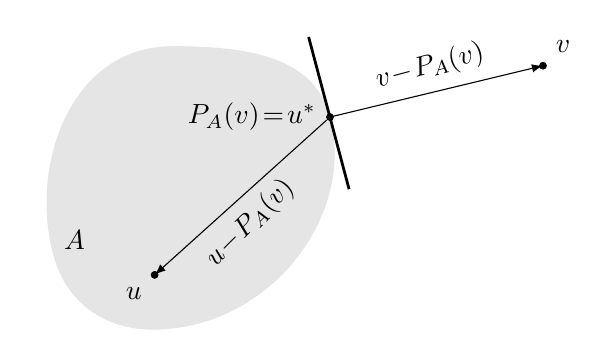
\begin{tikzpicture}[yscale=0.9,bullet/.style={circle,fill,inner sep=1.00pt,node contents={}}]
 \draw[-latex] (0,0) node[bullet,label=left:{$P_A(\vecnot{v}) \!=\! \vecnot{u}^*$},alias=PC]  -- (15:2.8) node[midway,sloped,above=0.25mm] {$\vecnot{v}\!-\! P_A(\vecnot{v})$}
    node[bullet,label=above right:$\vecnot{v}$,alias=v];
\draw[-latex] (PC) -- ++ (-135:3.15) node[pos=0.55,below=0.25mm,sloped]{$\vecnot{u}\!-\! P_A(\vecnot{v})$}     node[bullet,label=below left:$\vecnot{u}$];
\fill[black,fill,opacity=0.1] (PC) to[out=105,in=0] ++ (-2,1) to[out=180,in=105] ++ (-1.5,-3)
 node[above right,opacity=1]{$A$} to[out=-75,in=180] ++ (1.25,-1) to[out=0,in=-75] node[sloped, inner xsep=10mm, inner ysep=0, opacity=1, fill=black, pos=0.999] {} cycle;
\end{tikzpicture}
\caption{Orthogonal projection of $\vecnot{v}$ onto closed convex set $A$. \label{fig:pocs}}
\end{figure}

\begin{remark}
If $A$ is compact, then the existence of the minimum (for any norm) is given by topology because $\| \vecnot{v} - \vecnot{u} \|$ is continuous in $\vecnot{u}$.
Similarly, if both $\vecnot{u}$ and $\vecnot{u}'$ achieve the minimum distance $d$, then the convexity of the norm implies that the line segment between them also achieves the minimum distance. 
This implies that the closed ball of radius $d$ in $V$ contains a line segment on its boundary but one can use the Cauchy-Schwarz inequality to show this is impossible.
\end{remark}

The following theorem instead uses vector space methods to establish the same result for all closed convex $A$.

\begin{theorem}
\label{theorem:HilbertProjectionTheorem} For Hilbert space $V$, the orthogonal projection of $\vecnot v \in V$ onto a closed convex set $A\subseteq V$ exists and is unique.
\end{theorem}
\begin{proof}

Let $d=\inf_{\vecnot u\in A}\left\Vert \vecnot u-\vecnot v\right\Vert$ be the infimal distance between $\vecnot v$ and the set $A$.
Next, consider any sequence $\vecnot u_{1},\vecnot u_{2},\ldots\in A$ that achieves the infimum so that
\[
\lim_{n\rightarrow\infty}\left\Vert \vecnot u_{n}-\vecnot v\right\Vert =d.
\]
Since $A$ is complete, the next step is showing that this sequence is Cauchy. The parallelogram law states that $\left\Vert x-y\right\Vert ^{2}=2\left\Vert x\right\Vert ^{2}+2\left\Vert y\right\Vert ^{2}-\left\Vert x+y\right\Vert ^{2}$ and applying this to $\vecnot{x}=\vecnot{v}-\vecnot u_{n}$ and $\vecnot{y}=\vecnot{v}-\vecnot u_{m}$ gives
\begin{align*}
\left\Vert \vecnot u_{m}-\vecnot u_{n}\right\Vert ^{2} & =\left\Vert \left(\vecnot v-\vecnot u_{n}\right)-\left(\vecnot v-\vecnot u_{m}\right)\right\Vert ^{2}\\
 & =2\left\Vert \vecnot v-\vecnot u_{n}\right\Vert ^{2}+2\left\Vert \vecnot v-\vecnot u_{m}\right\Vert ^{2}-\left\Vert \left(\vecnot v-\vecnot u_{n}\right)+\left(\vecnot v-\vecnot u_{m}\right)\right\Vert ^{2}\\
 & =2\left\Vert \vecnot v-\vecnot u_{n}\right\Vert ^{2}+2\left\Vert \vecnot v-\vecnot u_{m}\right\Vert ^{2}-4\left\Vert \vecnot v-\frac{\vecnot u_{n}+\vecnot u_{m}}{2}\right\Vert ^{2}\\
 & \leq2\left\Vert \vecnot v-\vecnot u_{n}\right\Vert ^{2}+2\left\Vert \vecnot v-\vecnot u_{m}\right\Vert ^{2}-4d^{2}
\end{align*}
because the convexity of $A$ implies $\frac{\vecnot u_{n}+\vecnot u_{m}}{2}\in A$ and therefore $\left\Vert \vecnot v-\frac{\vecnot u_{n}+\vecnot u_{m}}{2}\right\Vert ^{2}\geq d^{2}$. Since the limit of the RHS (as $m,n\rightarrow\infty$) equals $0$, we find that the sequence $\vecnot u_{n}$ is Cauchy and therefore the limit $\vecnot u^{*}$ must exist. Since $\vecnot u_{n}\in A$ and $A$ is closed, we also see that $\vecnot u^{*}\in A$. Therefore, the infimum is achieved as a minimum.

Uniqueness can be seen by assuming instead that $\vecnot u_{m},\vecnot u_{n}$ are two elements in $A$ which are both at a distance $d$ from $\vecnot v$. Then, the above derivation shows that $\left\Vert \vecnot u_{m}-\vecnot u_{n}\right\Vert ^{2}\leq0$. Therefore, they are the same point.
\end{proof}

\begin{remark}
The same result holds for norm projections in many other Banach spaces including $L^{p}$ and $\ell^{p}$ for $1<p<\infty$. In general, it is required that the Banach space be strictly convex (for uniqueness) and reflexive (for existence).
\end{remark}



Earlier in this chapter, we studied the equivalence between the orthogonality and Hilbert-space projections onto subspaces.
The following result can be seen as a generalization of that result to Hilbert-space projections onto convex sets.

\begin{theorem}
\label{theorem:convex_proj_lt0}
For any $\vecnot{v} \notin A$, a necessary and sufficient condition for $\vecnot{u}^* = P_A (\vecnot{v})$ is that $\Real \langle \vecnot{v}-\vecnot{u}^* \,|\, \vecnot{u}-\vecnot{u}^* \rangle \leq 0$ for all $\vecnot{u}\in A$.
\end{theorem}
\begin{proof}
Let $\vecnot{u}^* = P_A (\vecnot{v})$ be the unique projection of $\vecnot{v}$ onto $A$.
For all $\vecnot{u} \in A$ %satisfying $\vecnot{u} \neq \vecnot{u}^*$
and any $\alpha\in (0,1)$, observe that $\vecnot{u}'=(1-\alpha) \vecnot{u}^* + \alpha \vecnot{u} = \vecnot{u}^* + \alpha (\vecnot{u}-\vecnot{u}^*)\in A$ due to convexity.
The optimality of $\vecnot{u}^*$ implies that
\begin{align*}
\| \vecnot{v}-\vecnot{u}^* \|^2
&\leq \| \vecnot{v}- \vecnot{u}' \|^2 \\
&\leq \| \vecnot{v}- \vecnot{u}^* - \alpha (\vecnot{u}-\vecnot{u}^*) \|^2 \\
&= \| \vecnot{v} - \vecnot{u}^* \|^2 + \alpha^2 \| \vecnot{u} - \vecnot{u}^* \|^2 - 2 \alpha \Real \langle v-\vecnot{u}^* \,|\, \vecnot{u}-\vecnot{u}^* \rangle. 
\end{align*}
Thus, $\Real \langle v-\vecnot{u}^* \,|\, \vecnot{u}-\vecnot{u}^* \rangle \leq \frac{\alpha}{2} \| \vecnot{u} - \vecnot{u}^* \|^2$.
One can establish necessity by taking the limit as $\alpha \to 0$.
For sufficiency, we assume $\Real \langle \vecnot{v}-\vecnot{u}^* | \vecnot{u}-\vecnot{u}^* \rangle \leq 0$ and we write
\begin{align*}
\| \vecnot{v}-\vecnot{u} \|^2 &- \| \vecnot{v} - \vecnot{u}^* \|^2
= \| (\vecnot{v} - \vecnot{u}^*) - (\vecnot{u} - \vecnot{u}^*) \|^2 - \|\vecnot{v} - \vecnot{u}^* \|^2 \\
&= \| \vecnot{v}-\vecnot{u}^* \|^2 + \| \vecnot{u} -\vecnot{u}^* \| ^2 - 2 \Real \langle v-\vecnot{u}^* \,|\, \vecnot{u}-\vecnot{u}^* \rangle - \|\vecnot{v}-\vecnot{u}^* \|^2 \\
&\geq 0.
\end{align*}
Thus, $\| \vecnot{v}-\vecnot{u} \|^2 \geq \| \vecnot{v} - \vecnot{u}^* \|^2$ for all $\vecnot{u} \in A$ and $\vecnot{u}^* = P_A (\vecnot{v})$.
\end{proof}

\subsection{Projection Properties and Examples}

Let $A$ be a closed convex subset of a Hilbert space $V$ over $\RealNumbers$.
By drawing a simple picture (e.g., see Figure~\ref{fig:pocs}), one can see that projecting $\vecnot{v}$ onto $A$ is an operation that is translation invariant.
Specifically, this means that translating the set $A$ and the vector $\vecnot v$ by the same vector $\vecnot v_{0}$ results in an output that is also translated by $\vecnot v_{0}$.
Mathematically, this means that, for all $\vecnot v,\vecnot v_{0}\in V$, the projection onto $V$ satisfies
\begin{align*}
P_{A+\vecnot v_{0}}(\vecnot v+\vecnot v_{0}) & =\arg\min_{\vecnot u\in A+\vecnot v_{0}}\left\Vert \vecnot u-\vecnot v-\vecnot v_{0}\right\Vert \nonumber \\
 & =\vecnot v_{0}+\arg\min_{\vecnot u'\in A}\left\Vert (\vecnot u'+\vecnot v_{0})-\vecnot v-\vecnot v_{0}\right\Vert \nonumber \\
 & =\vecnot v_{0}+\arg\min_{\vecnot u'\in A}\left\Vert \vecnot u'-\vecnot v\right\Vert \nonumber \\
 & =\vecnot v_{0}+P_{A}(\vecnot v).\label{eq:proj_trans}
\end{align*}
This also leads to the following trick. If a projection is easy when the set is centered, then one can: (i) translate the problem so that the set is centered, (ii) project onto the centered set, and (iii) translate back. 

Using the best approximation theorem, it is easy to verify that the orthogonal projection of $\vecnot v\in V$ onto a one-dimensional subspace $W=\text{span}(\vecnot w)$ is given by
\[
P_{W}(\vecnot v)=\frac{\left\langle \vecnot v|\vecnot w\right\rangle }{\left\Vert \vecnot w\right\Vert ^{2}}\vecnot w.
\]

A \defn{vector space}{hyperplane} is a closed subspace of $U \subset V$ that satisfies a single linear equality of the form $\left\langle \vecnot v|\vecnot w\right\rangle =0$ for all $\vecnot{v}\in U$.
Such a subspace is said to have co-dimension one (e.g., if $\dim(V)=n$, then $\dim(U) = n-1$). Equivalently, $U$ can be seen as the orthogonal complement of a one-dimensional subspace (e.g., $U=W^{\perp}$).
Thus, we can write
\[
P_{U}(\vecnot v)=P_{W^{\perp}}(\vecnot v)=\vecnot v-\frac{\left\langle \vecnot v|\vecnot w\right\rangle }{\left\Vert \vecnot w\right\Vert ^{2}}\vecnot w.
\]

Similarly, a linear equality such as $\langle\vecnot v|\vecnot w\rangle=c$, where $\vecnot v_{0}$ is any vector in $V$ satisfying $\langle\vecnot v_{0}|\vecnot w\rangle=c$,  defines an \defn{vector space}{affine hyperplane}.
This is the shifted subspace $U+\vecnot v_{0}$ of co-dimension one because 
\[
\langle\vecnot v|\vecnot w\rangle=\langle\vecnot u+\vecnot v_{0}|\vecnot w\rangle=\langle\vecnot u|\vecnot w\rangle+\langle\vecnot v_{0}|\vecnot w\rangle=0+c=c.
\]
Thus, we can project onto $U+\vecnot{v_{0}}$ by translating, projecting, and then translating back. This gives
\begin{equation*}
P_{U+\vecnot v_{0}}(\vecnot v)=\left((\vecnot v-\vecnot v_{0})-\frac{\left\langle \vecnot v-\vecnot v_{0}|\vecnot w\right\rangle }{\left\Vert \vecnot w\right\Vert ^{2}}\vecnot w\right)+\vecnot v_{0}=\vecnot v-\frac{\left\langle \vecnot v|\vecnot w\right\rangle -c}{\left\Vert \vecnot w\right\Vert ^{2}}\vecnot w,\label{eq:proj_lin_eq}
\end{equation*}
which does not depend on the choice of $\vecnot v_{0}$.

Next, let $H$ be the subset of $\vecnot v\in V$ satisfying the linear inequality $\langle\vecnot v|\vecnot w\rangle\geq c$. Then, $H$ is a closed convex set known as a \defn{inner-product space}{half space}. For any $\vecnot v\in H$, we have $P_{H}(\vecnot v)=\vecnot v$ and, for any $\vecnot v\notin H$, we have $P_{H}(\vecnot v)=P_{U+\vecnot v_{0}}(\vecnot v)$ because the closest point must lie on the separating hyperplane and achieve the inequality with equality. For any $\vecnot v\in H$, one can put these together to see that
\begin{equation}
P_{H}(\vecnot v)=\begin{cases}
\vecnot v & \text{if }\langle\vecnot v|\vecnot w\rangle\geq c\\
\vecnot v-\frac{\left\langle \vecnot v|\vecnot w\right\rangle -c}{\left\Vert \vecnot w\right\Vert ^{2}}\vecnot w & \text{if }\langle\vecnot v|\vecnot w\rangle<c.
\end{cases}\label{eq:proj_ineq}
\end{equation}

\begin{theorem} \label{theorem:convex_point_set_hyperplane}
Let $V$ be a Hilbert space over $\RealNumbers$ and $A\subset V$ be a closed convex set.
For any $\vecnot{v} \notin A$, there is an affine hyperplane $U' = \{ \vecnot{u} \in V \,|\, \langle \vecnot{u} | \vecnot{w} \rangle = c \}$ (defined by $\vecnot{w} \in V$ and $c\in \RealNumbers$) such that $\langle \vecnot{v} | \vecnot{w} \rangle < c$ and $\langle \vecnot{u} | \vecnot{w} \rangle \geq c$ for all $\vecnot{u} \in A$.
\end{theorem}

\begin{proof}
Let $\vecnot{u}^* = P_A (\vecnot{v})$ be the orthogonal projection of $\vecnot{v}$ onto $A$ and define $\vecnot{w} = \vecnot{u}^* - \vecnot{v}$ and $c= \langle \vecnot{u}^* | \vecnot{w} \rangle$.
From Theorem~\ref{theorem:convex_proj_lt0}, we see that $\langle \vecnot{v}-\vecnot{u}^* | \vecnot{u}-\vecnot{u}^* \rangle \leq 0$ for all $\vecnot{u} \in A$.
Thus, for all $\vecnot{u}\in A$, we have
\begin{align*}
\langle \vecnot{u} | \vecnot{w} \rangle
&= \langle \vecnot{w} | \vecnot{u} \rangle
= \langle \vecnot{u}^* - \vecnot{v} | \vecnot{u} \rangle
= - \langle \vecnot{v} - \vecnot{u}^* | \vecnot{u} \rangle \\
&\stackrel{(a)}{\geq} - \langle \vecnot{v} - \vecnot{u}^* | \vecnot{u}^* \rangle
= \langle \vecnot{u}^* - \vecnot{v} | \vecnot{u}^* \rangle
\\
&= \langle \vecnot{w} | \vecnot{u}^* \rangle
= \langle \vecnot{u}^* | \vecnot{w} \rangle
= c,
\end{align*}
where $(a)$ follows from $\langle \vecnot{v}-\vecnot{u}^* | \vecnot{u}-\vecnot{u}^* \rangle \leq 0$ for all $\vecnot{u} \in A$.
For $\langle \vecnot{v} | \vecnot{w} \rangle$, we observe that together, $\vecnot{u}^* \in A$ and $\vecnot{v} \notin A$, imply that
\begin{align*}
0 &< \| \vecnot{u}^* - \vecnot{v} \|^2
= \langle \vecnot{u}^* - \vecnot{v} | \vecnot{u}^* - \vecnot{v} \rangle \\
&= \langle \vecnot{u}^* | \vecnot{u}^* - \vecnot{v} \rangle - \langle  \vecnot{v} | \vecnot{u}^* - \vecnot{v} \rangle
= c - \langle  \vecnot{v} | \vecnot{u}^* - \vecnot{v} \rangle,
\end{align*}
which shows that $\langle \vecnot{v} | \vecnot{w} \rangle < c$ and completes the proof.
\end{proof}

\begin{theorem}
Let $V$ be Hilbert space over $\RealNumbers$ and $A \subset V$ be a closed convex set.
Then, $A$ equals the intersection of a set of half spaces.
\end{theorem}

\begin{proof}
Let $\mathcal{H}$ be the set of all half spaces in $V$ and let $\mathcal{G} = \{ H\in \mathcal{H} \,|\, A \subseteq H \}$  be the subset of half spaces containing $A$.
For example, consider the half spaces defined by tangent planes passing through points on the boundary of $A$.
Let $B= \cap_{H\in \mathcal{G}} H$ be the intersection of all the half spaces in $\mathcal{G}$.
Since each half space contains $A$, it is clear that $A\subseteq B$.
To show that $A = B$, we will show that $(x\notin A) \to (x\notin B)$.
If $x \notin A$, then Theorem~\ref{theorem:convex_point_set_hyperplane} shows that there is an affine hyperplane that separates $x$ from $A$ and an associated half space $G$ that contains $A$ but not $x$.
Since $G$ contains $A$, it follows that $G \in \mathcal{G}$.
But, $x \notin G$ implies $x \notin B$ because $B$ is the intersection of the half spaces in $\mathcal{G}$. 
This completes the proof.
\end{proof}

\subsection{Minimum Distance Between Two Convex Sets}

Now, consider the smallest distance between two disjoint closed convex sets $A,B\subseteq V$. In this case, a unique solution may exist but a some things can go wrong. If the two sets are not strictly convex (e.g., consider two squares), then it is clearly possible for their to multiple pairs of points that achieve the minimum distance. Even if the two sets are strictly convex, one may find that the infimum is achieved as the points wander off to infinity. For example, consider the strictly convex hyperbolic sets $A=\left\{ (x,y)|x^{2}-y^{2}\geq1,x>0\right\} $ and $B=\left\{ (x,y)|y^{2}-x^{2}\geq1,y\geq0\right\} $. These two sets share the line $x=y>0$ as an asymptote, so their infimal distance is 0.

To understand this behavior, we first note that the distance $f\left(\vecnot u,\vecnot v\right)=\left\Vert \vecnot u-\vecnot v\right\Vert $ is a convex function on the convex product set $A\times B$.
It follows that any local minimum value is a global minimum value distance.
\begin{theorem}
\label{thm:MinDistTwoConvexSet} Let $V$ be a Hilbert space and consider the infimal distance
\[
d=\inf_{\vecnot u\in A,\vecnot v\in B}\left\Vert \vecnot u-\vecnot v\right\Vert 
\]
between two disjoint closed convex sets $A,B\subseteq V$.
If either set is compact, then the infimum is achieved.
If the infimum is achieved and either set is strictly convex, then the minimizing points $\vecnot u^{*},\vecnot v^{*}$ are unique.
\end{theorem}

\begin{proof}
Consider any sequence $(\vecnot u_{1},\vecnot v_{1}),(\vecnot u_{2},\vecnot v_{2}),\ldots\in A\times B$ that satisfies
\[
\lim_{n\rightarrow\infty}\left\Vert \vecnot u_{n}-\vecnot v_{n}\right\Vert =d.
\]
If $B$ is compact, then there is a subsequence $\vecnot v_{n_{j}}$ that converges to some $\vecnot v^{*}\in B$.
Since $\| P_A (\vecnot{v}_n)-\vecnot v_{n} \| \leq \|\vecnot u_{n}-\vecnot v_{n}\| $, we can replace $\vecnot u_{n_{j}}$ by $P_A (\vecnot{v}_{n_j})$ and still achieve the infimum.
The continuity of $P_A$ also shows that $u_{n_{j}} \to \vecnot{u}^* = P_A (\vecnot{v}^*)$ and this implies $\| \vecnot{u}^* - \vecnot{v}^* \| = d$.
Also, $P_B (\vecnot{u}^*) = \vecnot{v}^*$ because $\vecnot{v}^*$ is the unique closest point in $B$ to $\vecnot{u}^*$.
Notice that $\vecnot v^{*}$ may not be unique (due to the subsequence construction) and, thus, the pair $(\vecnot{u}^*,\vecnot{v}^*)$ is not unique in general.

Since $\left\Vert \vecnot u-\vecnot v\right\Vert $ is a convex function on the convex product set $A\times B$, there is a (possibly empty) convex set of minimizers

\[
M=\left\{ (\vecnot u,\vecnot v)\in A\times B\;\big|\;\left\Vert \vecnot u-\vecnot v\right\Vert =d\right\} .
\]
Also, each component of the $(\vecnot{u},\vecnot{v})$ points in $M$ must lie on the boundary of its set because otherwise one could reduce the smallest distance by moving one point along the minimum distance line towards the boundary. Now, suppose that (i) $A$ is strictly convex and (ii) $M$ contains more than one pair of minimizers. Then, condition (ii) implies that there must be two boundary points $\vecnot u_{1},\vecnot u_{2}\in\partial A$ such that $\alpha\vecnot u_{1}+(1-\alpha)\vecnot u_{2}\in\partial A$ for $\alpha\in[0,1]$. But this contradicts condition (i) and shows that, if $A$ is strictly convex, then there is at most one pair $(\vecnot u^{*},\vecnot v^{*})\in M$ of minimizing points.
\end{proof}

\begin{remark}
Finding the minimum distance between two disjoint closed convex sets $A,B\subseteq V$ is a classic problem that is solved nicely by the idea of alternating minimization. Let $\vecnot v_{0}\in B$ be an arbitrary initial point and define
\begin{align*}
\vecnot u_{n+1} & =\arg\min_{\vecnot u\in A}\left\Vert \vecnot u-\vecnot v_{n}\right\Vert \\
\vecnot v_{n+1} & =\arg\min_{\vecnot v\in B}\left\Vert \vecnot u_{n+1}-\vecnot v\right\Vert .
\end{align*}
Notice that the sequence $d_{n}=\left\Vert \vecnot u_{n}-\vecnot v_{n}\right\Vert $ is non-increasing and must therefore have a limit.
By adapting the previous proof, one can show that, if either set is compact, then the sequence $(\vecnot u_{n},\vecnot v_{n})$ converges to a pair of vectors that minimize the distance. % cite []Bauschke, Finding Best Approx. Pairs]
%Variations of this approach can even be useful when $A\cap B\neq\emptyset$.
%In this case, sequence $\vecnot v_{n}$ converges weakly to some point $\vecnot v\in A\cap B$.
\end{remark}

\begin{theorem}
Let $V$ be a Hilbert space over $\RealNumbers$ and $A,B$ be disjoint closed convex subsets of $V$.
If either set is compact, then there is an affine hyperplane $\{ \vecnot{a} \in V \,|\, \langle \vecnot{a} | \vecnot{w} \rangle = c \}$ (defined by $\vecnot{w} \in V$ and $c\in \RealNumbers$) such that $\langle \vecnot{u} | \vecnot{w} \rangle > c$ for all $\vecnot{u} \in A$ and $\langle \vecnot{u} | \vecnot{w} \rangle < c$ for all $\vecnot{u} \in B$.
\end{theorem}
\begin{proof}
Applying Theorem~\ref{thm:MinDistTwoConvexSet} gives a pair of points $(\vecnot{u}^*,\vecnot{v}^*) \in A \times B$ that minimize the distance and satisfy $\vecnot{u}^* = P_A (\vecnot{v}^*)$ and $\vecnot{v}^* = P_B (\vecnot{u}^*)$.
Applying Theorem~\ref{theorem:convex_point_set_hyperplane} to $P_A (\vecnot{v}^*)$ shows that $\langle \vecnot{u} | \vecnot{u}^* - \vecnot{v}^* \rangle \geq \langle \vecnot{u}^* | \vecnot{u}^* - \vecnot{v}^* \rangle$ for all $\vecnot{u} \in A$.
Similarly, applying Theorem~\ref{theorem:convex_point_set_hyperplane} to $P_B (\vecnot{u}^*)$ shows that $\langle \vecnot{v} | \vecnot{v}^* - \vecnot{u}^* \rangle \geq \langle \vecnot{v}^* | \vecnot{v}^* - \vecnot{u}^* \rangle$ for all $\vecnot{v} \in B$.
Negating this gives $\langle \vecnot{v} | \vecnot{u}^* - \vecnot{v}^* \rangle \leq \langle \vecnot{v}^* | \vecnot{u}^* - \vecnot{v}^* \rangle$.
Now, we observe that  $\langle \vecnot{u}^* | \vecnot{u}^* - \vecnot{v}^* \rangle - \langle \vecnot{v}^* | \vecnot{u}^* - \vecnot{v}^* \rangle = \| \vecnot{u}^* - \vecnot{v}^* \|^2 > 0$ because $\vecnot{u}^* \neq \vecnot{v}^*$.
Thus, we can choose $\vecnot{w} = \vecnot{u}^* - \vecnot{v}^*$ and $c=\frac{1}{2}(\langle \vecnot{u}^* | \vecnot{u}^* - \vecnot{v}^* \rangle + \langle \vecnot{v}^* | \vecnot{u}^* - \vecnot{v}^* \rangle)$  to guarantee that $\langle \vecnot{u} | \vecnot{w} \rangle > c$ for all $\vecnot{u} \in A$ and $\langle \vecnot{u} | \vecnot{w} \rangle < c$ for all $\vecnot{u} \in B$.
\end{proof}

\iffalse
\subsection{Alternating Projections}

Another classic result for projections in a Hilbert space is that alternating between projections onto multiple subspaces leads to a projection onto the intersection of all the subspaces.
\begin{lemma}
Let $V$ be a separable Hilbert space and $P_{W}$ be a projection onto the closed subspace $W\subset V$. Then, $\left\Vert P_{W}\vecnot v_{n}\right\Vert \rightarrow\left\Vert \vecnot v_{n}\right\Vert \rightarrow d$ implies that $\vecnot v_{n}\rightarrow\vecnot v\in W$. (not correct) Need to show vector is decreasing in some sense!!! For any projection-like $T$, $\vecnot v_{n}=T^{n}\vecnot v_{0}$. non-expansive. If not fixed point, then coefficients reduced in some basis (i.e., cannot wander off to new basis elements)
\end{lemma}
\begin{proof}
Let $\vecnot w_{1},\vecnot w_{2},\ldots$ be a orthonormal basis for $W$ Orthogonal decomposition of projection shows that
\end{proof}
\fi
